%%%%%%%%%%%%%%%%%%%%%%%%%%%%%%%%%%%%%%%%%
% a0poster Landscape Poster
% LaTeX Template
% Version 1.0 (22/06/13)
%
% The a0poster class was created by:
% Gerlinde Kettl and Matthias Weiser (tex@kettl.de)
% 
% This template has been downloaded from:
% http://www.LaTeXTemplates.com
%
% License:
% CC BY-NC-SA 3.0 (http://creativecommons.org/licenses/by-nc-sa/3.0/)
%
%%%%%%%%%%%%%%%%%%%%%%%%%%%%%%%%%%%%%%%%%

%----------------------------------------------------------------------------------------
%	PACKAGES AND OTHER DOCUMENT CONFIGURATIONS
%----------------------------------------------------------------------------------------

\documentclass[a0,landscape]{a0poster}

\usepackage{multicol} % This is so we can have multiple columns of text side-by-side
\columnsep=100pt % This is the amount of white space between the columns in the poster
\columnseprule=3pt % This is the thickness of the black line between the columns in the poster

\usepackage[svgnames]{xcolor} % Specify colors by their 'svgnames', for a full list of all colors available see here: http://www.latextemplates.com/svgnames-colors

\usepackage{times} % Use the times font
%\usepackage{palatino} % Uncomment to use the Palatino font

\usepackage{graphicx} % Required for including images
\graphicspath{{figures/}} % Location of the graphics files
\usepackage{booktabs} % Top and bottom rules for table
\usepackage[font=small,labelfont=bf]{caption} % Required for specifying captions to tables and figures
\usepackage{amsfonts, amsmath, amsthm, amssymb} % For math fonts, symbols and environments
\usepackage{wrapfig} % Allows wrapping text around tables and figures
\usepackage{hyperref}
\begin{document}

%----------------------------------------------------------------------------------------
%	POSTER HEADER 
%----------------------------------------------------------------------------------------

% The header is divided into three boxes:
% The first is 55% wide and houses the title, subtitle, names and university/organization
% The second is 25% wide and houses contact information
% The third is 19% wide and houses a logo for your university/organization or a photo of you
% The widths of these boxes can be easily edited to accommodate your content as you see fit

\begin{minipage}[b]{0.55\linewidth}
\veryHuge \color{NavyBlue} \textbf{JamBand: a Human-Robot Interactive Band} \color{Black}\\ % Title
\Huge\textit{EE183}\\[1cm] % Subtitle
\huge \textbf{Wilson Chang}\\ % Author(s)
\huge University of California, Los Angeles\\ % University/organization
\end{minipage}
%
\begin{minipage}[b]{0.25\linewidth}
\color{DarkSlateGray}\Large \textbf{Contact Information:}\\
HSEAS\\ % Address
UCLA\\
7400 Boelter Hall, Los Angeles, CA 90095 \\\\

Email: \texttt{ckwojai@ucla.edu}\\ % Email address
Website: \href{https://github.com/ckwojai/EE183\_JamBand}{https://github.com/ckwojai/EE183\_JamBand}\\ % Phone number

\end{minipage}
%
\begin{minipage}[b]{0.19\linewidth}

\includegraphics[width=20cm]{logo.jpg} % Logo or a photo of you, adjust its dimensions here
\end{minipage}

\vspace{1cm} % A bit of extra whitespace between the header and poster content

%----------------------------------------------------------------------------------------

\begin{multicols}{4} % This is how many columns your poster will be broken into, a poster with many figures may benefit from less columns whereas a text-heavy poster benefits from more

%----------------------------------------------------------------------------------------
%	ABSTRACT
%----------------------------------------------------------------------------------------

\color{Navy} % Navy color for the abstract

\begin{abstract}
Our goal was to build a musical “jam band” driven by two ESP8266 micro-controllers, utilizing sensors and actuators. The main challenges in this project includes 1) composing music with Buzzer and Servo, 2) communication and synchronization between the two micro-controllers, and 3) Deploy the project online. We solved these problems using 1) note-frequency matching and delay time control, 2) Serial communication, and 3) Port-forwarding. In this poster, we will guide your through our solutions. 
\end{abstract}

%----------------------------------------------------------------------------------------
%	INTRODUCTION
%----------------------------------------------------------------------------------------

\color{SaddleBrown} % SaddleBrown color for the introduction

\section*{Introduction}
In this project, we build our JamBand with two micro-controller with Buzzer and Servo mimicking the trumpet and drumstick. We also incorporate ultrasonic sensor and touch sensor for human interaction with the band. A Web interface is also designed for use to access the autonomous mode of the band through Internet. 

%----------------------------------------------------------------------------------------
%	OBJECTIVES
%----------------------------------------------------------------------------------------

\color{DarkSlateGray} % DarkSlateGray color for the rest of the content

\section*{Music Composition}
In our project, two songs are composed, namely Twinkle Twinkle Little star and Row Row Row the boat. To code for the buzzer to sound like any music, we define a number of notes with its corresponding frequency. As shown below:
\begin{center}\vspace{1cm}
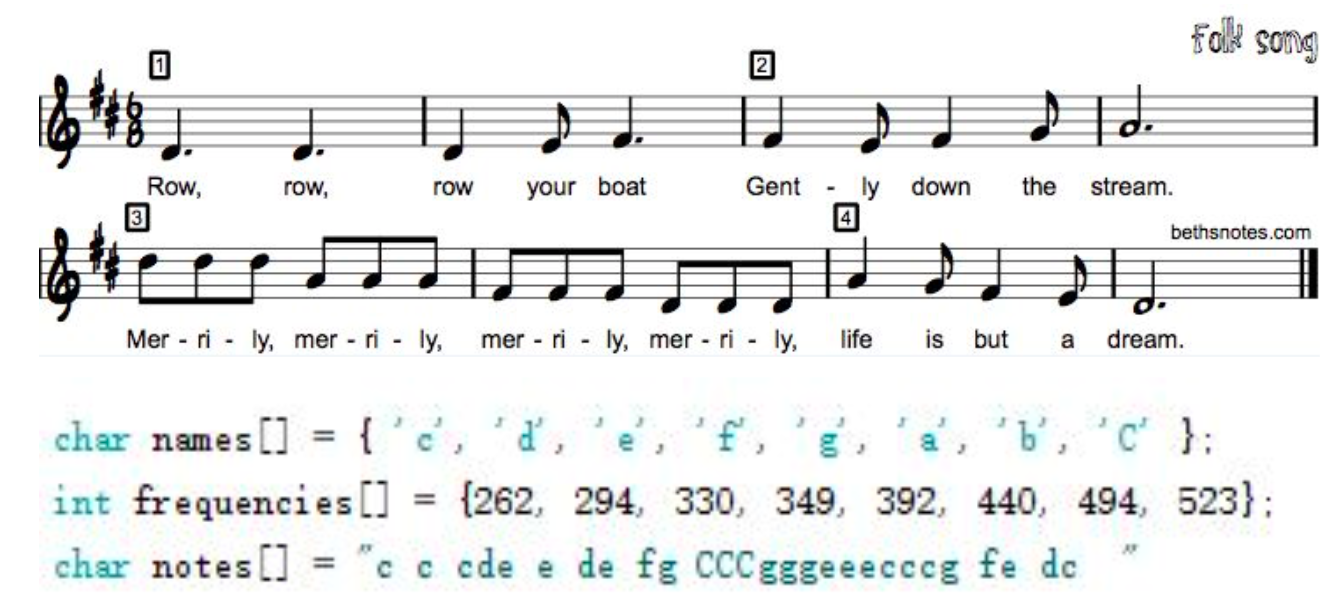
\includegraphics[width=0.8\linewidth]{compose}
\captionof{figure}{\color{Green} Figure caption}
\end{center}\vspace{1cm}
We then make sound with the buzzer using the corresponding frequency to match each note in the sheet. A duration is also added for the time length of each note. These two parameters are then pass to the Arduino function tone(frequency, duration) to let the buzzer make Sound. \par
As for the servo, it's better to code this together with the buzzer for synchronization purpose. We first need to determine the starting and ending angle for the servo. Fix the ending angle because that's where the stick hit the drum every time. Then program the delay as shown below, assume the initial configuration of servo is at starting angle,
\begin{enumerate}
\item Set the servo to the ending angle
\item Apply some delay too allow time for the servo to go to the ending angle
\item After the above appropriate delay, this is when the stick hit the drum
\item Start playing one note of the buzzer music
\item Set the servo back to starting angle, and apply some delay for it to get there
\item Repeat the above steps
\end{enumerate}
Note that there are two ways to set the duration for each stick hit: either by changing the starting angle or give it less delay time to go to starting angle (so that it's still on his way to starting angle when the next end angle command is already received). Both of these two methods are used in our program, it's also essential to parameterize these delays so that we can control the tempo of both instruments.

%----------------------------------------------------------------------------------------
%	MATERIALS AND METHODS
%----------------------------------------------------------------------------------------

\section*{Serial Communication}
After composing our music, we get both instruments to play in the same speed and note. However, there have to be some communication between these two instruments for them to know when and what music and tempo to play. We accomplished this with Serial Communication between the micro-controllers. \par
To establish the communication channel, we wire up Tx$\leftrightarrow$Tx and Rx$\leftrightarrow$Tx for the two micro-controllers. Now, one has to act as a sender and the other receiver. In our project, we arbitrarily chose the servo to be the sender.\par
Sender's job is easy, through Serial, send (print) a Ready signal R, followed by a Song signal S, and then a tempo Signal T. On the receiver side, three layers of if statement are constantly checking if there are anything in the Serial buffer (if (Serial.available()>0)) and read the message. Know the signals, it then set and play the song with the right tempo. 

%------------------------------------------------

\section*{Port Forwarding}
After robots are functioning properly, we started to think of a way to get our Robots online. We followed the tutorials online, and was able to set up ESP8266 to be a WIFI access point. However, user has to connect to the designated WIFI and command through a ugly User Interface. \par
In order to change this, we need to somehow get our Robot really online so we can have a separate more customizable page to control our robot. After some research, Port Forwarding seems to be a feasible solution. \par
To set things up, we first need to set our ESP8266 now to be a Workstation rather than an Access Point. This Workstation is connected to our Home Wifi given SSID and Password. We should now be able to access the control page if we are connected to our home WIFI. Now to get page entirely online, we need to use our Router IP address (since our router is connected to the Internet). \par
First we go to \url{http://www.whatsmyip.org} to get our Router IP. We then go to our router setting and look for Port Forwarding and fill in the according IP address and port (we define this in our Arduino code). As shown below,
\begin{center}\vspace{1cm}
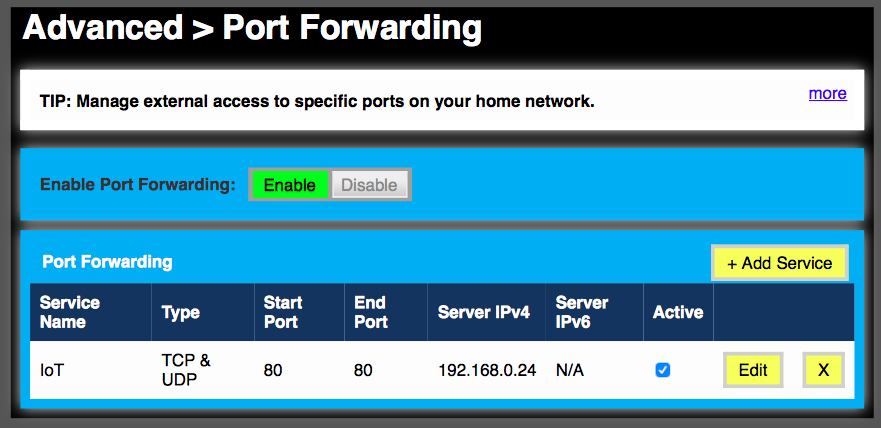
\includegraphics[width=0.8\linewidth]{pf}
\captionof{figure}{\color{Green} Port Forwarding in Router Setting}
\end{center}\vspace{1cm}
Now if we go to our router IP address, we should be able to get the control page from anywhere whether using WIFI or cellular data. All the above work makes this beautiful user interface possible:
\begin{center}\vspace{1cm}
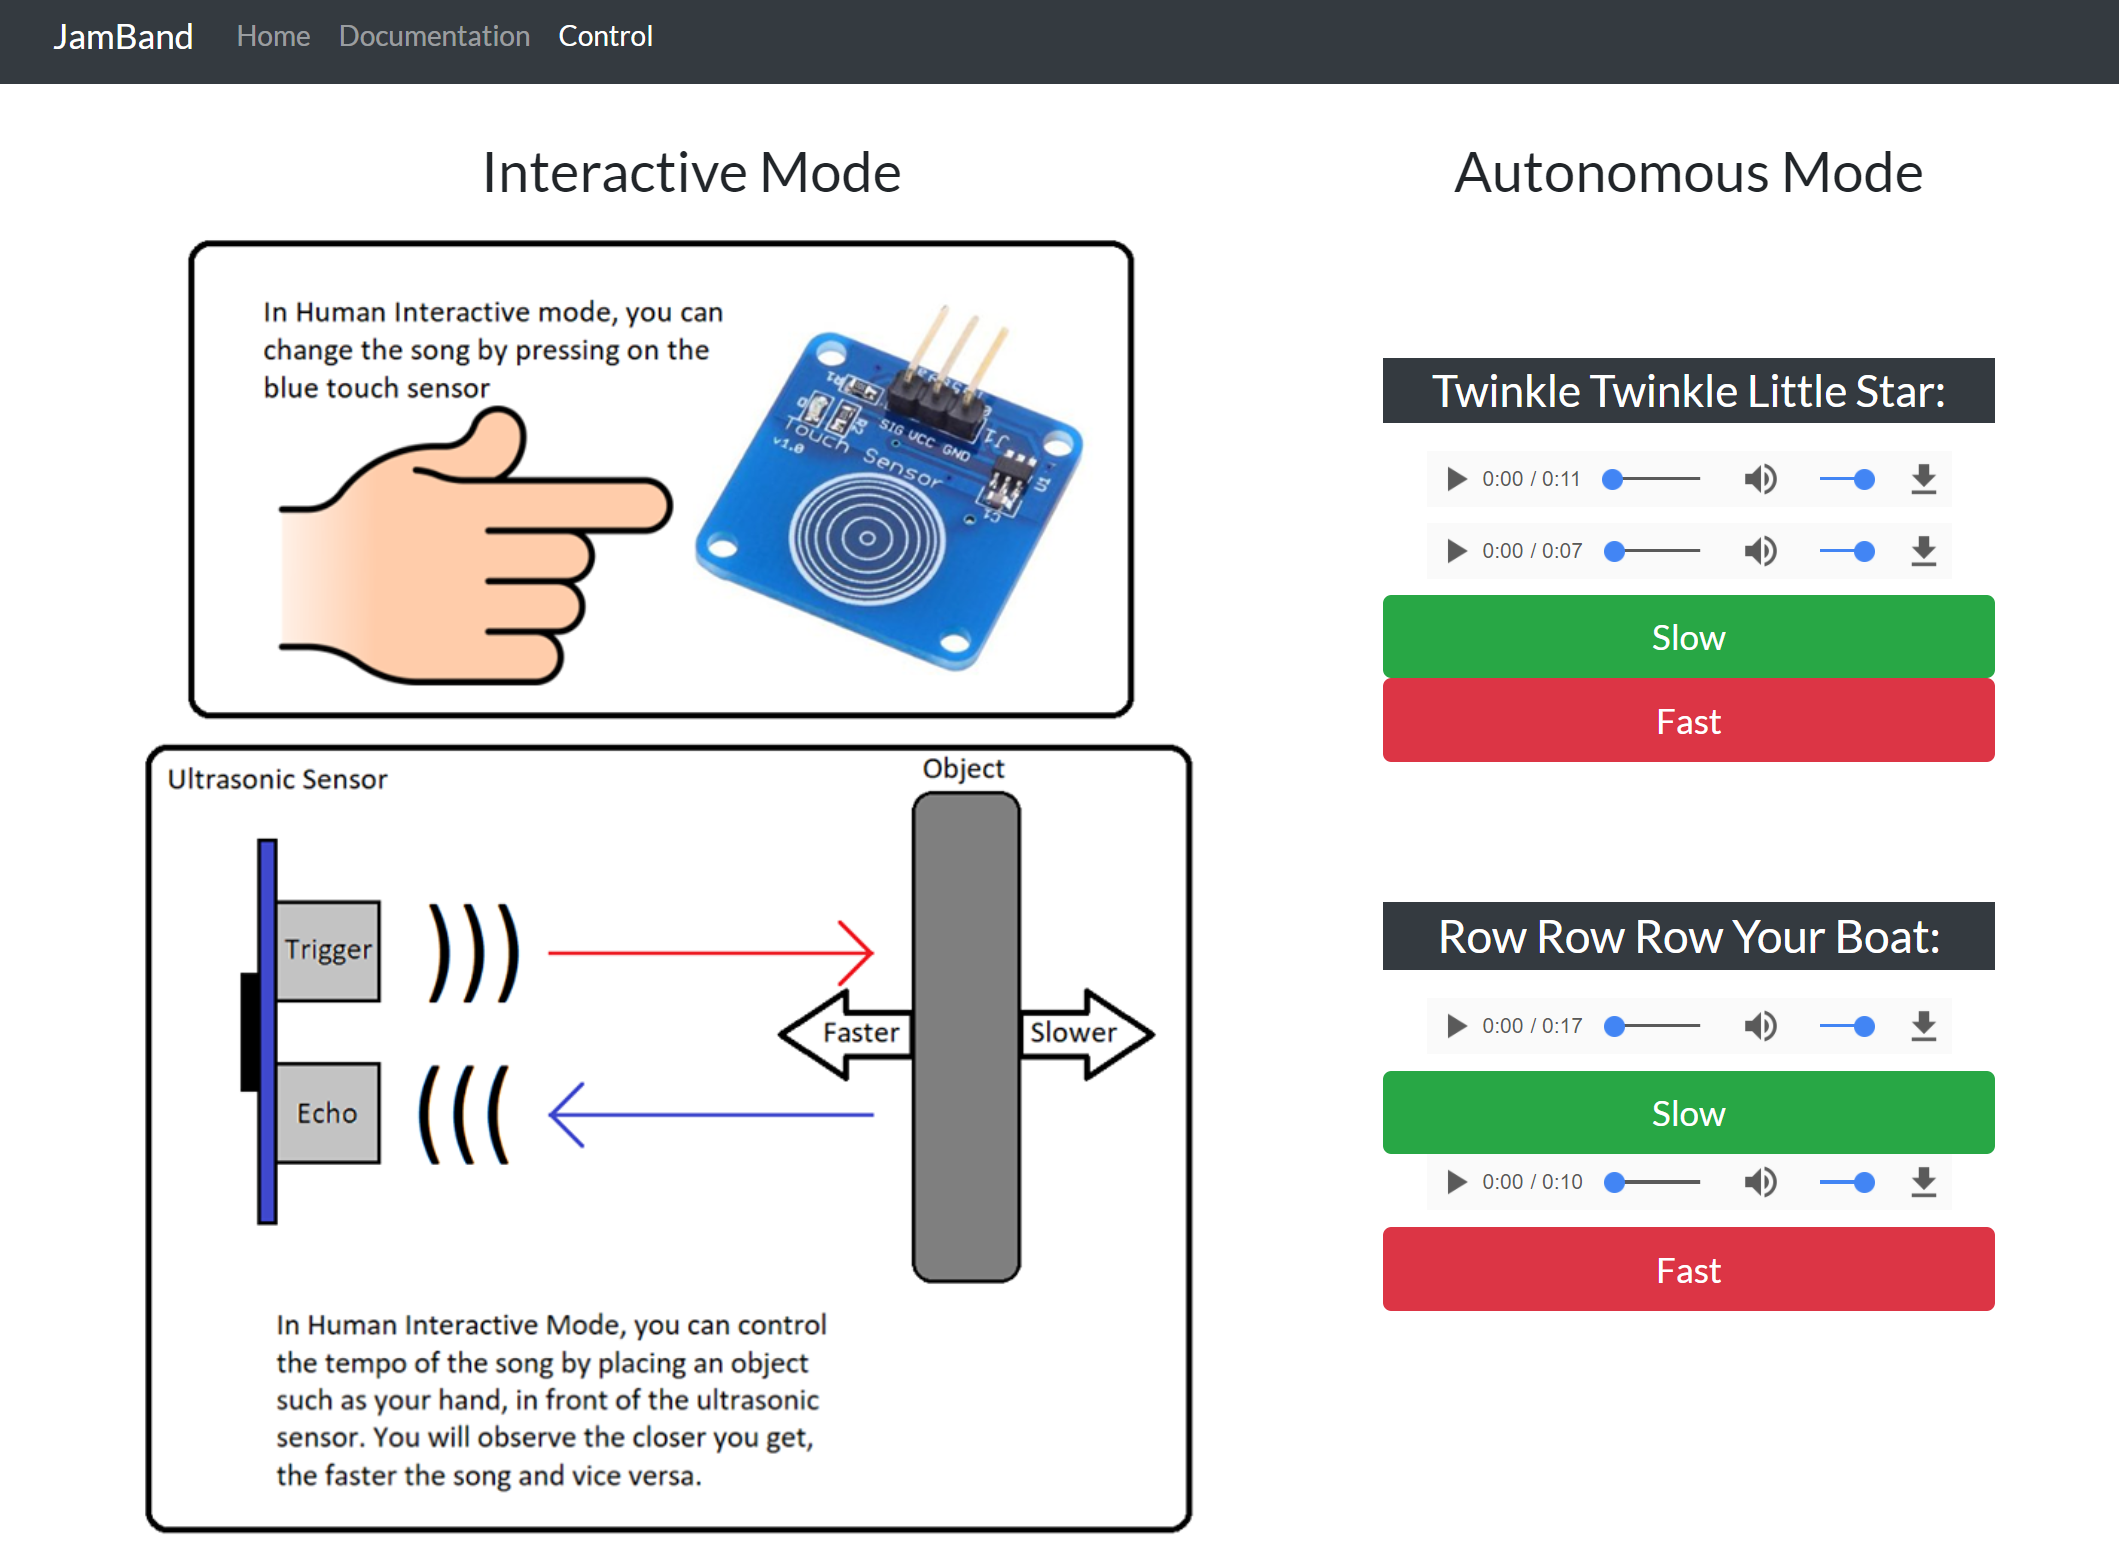
\includegraphics[width=0.8\linewidth]{website2}
\captionof{figure}{\color{Green} Our Awesome User Interface}
\end{center}\vspace{1cm}

%----------------------------------------------------------------------------------------
%	RESULTS 
%----------------------------------------------------------------------------------------
\section*{Potential Improvement}
I would like to mentions at last about some potential improvements of this project. As listed below,
\begin{enumerate}
\item The servo end angle consistency of the two songs. Since the two songs are composed by two teammates individually, the end angle are not the same. As a result, the drum has to move to the right position every time the song switched for the stick to hit the drum properly.
\item User interaction is not immediate. Since we programmed in each loop that the music is played for a 7-14 second. During the playing of the music, the sensors' value won't be measured and also the client request won't be accepted. This caused the problem that users has to interact with the Robot at the end of a loop cycle. 
\item To continue my first point, possible improvements can be made to divide the song playing function in a very small segments so that the loop still repeat in a reasonably short time to do all the instant measurement and web service. However, this maybe challenging as to parameterize the song with each loop variables.
\end{enumerate}

%----------------------------------------------------------------------------------------
%	CONCLUSIONS
%----------------------------------------------------------------------------------------

\section*{Conclusion}

\color{SaddleBrown} % SaddleBrown color for the conclusions to make them stand out
In this poster, we guided your through a detail problem solving process in our project, including Music Composition, Serial Communication, and Wireless setup. We also address some potential improvements of our project such as inconsistency of servo and immediate user interaction.
\color{DarkSlateGray} % Set the color back to DarkSlateGray for the rest of the content

 %----------------------------------------------------------------------------------------
%	REFERENCES
%----------------------------------------------------------------------------------------

\nocite{*} % Print all references regardless of whether they were cited in the poster or not
\bibliographystyle{plain} % Plain referencing style
\bibliography{sample} % Use the example bibliography file sample.bib

%----------------------------------------------------------------------------------------
%	ACKNOWLEDGMENTS
%----------------------------------------------------------------------------------------

\section*{Acknowledgments}
I would like to thank my EE183 Professor Mehta for this awesome project.
%----------------------------------------------------------------------------------------

\end{multicols}
\end{document}